\documentclass[bwprint]{gmcmthesis}
\usepackage[framemethod=TikZ]{mdframed}
\title{方形件组批及排样优化策略研究}
\baominghao{22103350008} %参赛队号
\schoolname{浙江大学}%学校名称
\membera{葛明阳} %队员A
\memberb{郑欣怡} %队员B
\memberc{董萌苇} %队员C
\begin{document}
\sloppy

 %生成标题
 \maketitle

 %填写摘要
\begin{abstract}
本文对方形件排样问题及订单组批问题建立\textbf{混合整数规划模型},通过设计构造\textbf{贪心算法},实现方形件排样优化和组批优化。针对题目数据集,得出完整的组批及排样方案,并以\textbf{数据表}、\textbf{效果图}等形式加以展示。最后,本文还将对完整算法的\textbf{合理性}、\textbf{求解有效性}、\textbf{复杂度}、\textbf{运行时间}进行分析讨论,并给出其程序源码。

\textbf{针对问题1},本文建立方形件排样优化问题\textbf{混合整数线性规划模型},采用\textbf{有限降序首次适应算法}对该问题进行求解。在\textbf{考虑产品项旋转}的情况下,使用\textbf{高度优先}及\textbf{左下优先(Bottom-Left,BL)}原则,得出方形件排样方案。该算法\textbf{空间复杂度}为$O(n)$,\textbf{最佳时间复杂度}为$O(n)$,\textbf{最坏时间复杂度}为$O(n^2)$。

针对该题目数据集,该算法所得排样方案的板材使用数量接近\textbf{商业矩形排样软件的非三阶段精确排样结果},且与理论最优值相差不大。该算法计算时间短,平均每个数据集计算时间不超过\textbf{200ms}。该题目中得到4套排样优化方案原始板材利用率分别为\textbf{94.93\%、93.12\%、95.15\%、94.08\%},原始板材使用个数分别为\textbf{88、89、88、87}片。

\textbf{针对问题2},本文在问题1的基础上建立订单组批优化问题\textbf{混合整数非线性规划模型},通过\textbf{两步优化}法,针对总板材利用率最高构造两层优化问题。本问设计适用于此问题的\textbf{优先搜索}算法,最终形成的组批方案及排样方案。

针对该题目数据集,该算法所得组批方案的原始板材使用数量接近\textbf{同时生产所有批次产品项时的排样所需的原始板材数量}。该算法计算时间短,在大量数据和复杂优化的情况下,该算法仍然可以保证针每个数据集计算时间不超过\textbf{20min},在较好情况计算时间不超过\textbf{10min}。该题目中得到5套组批及排样优化方案的材利用率分别为\textbf{79.23\%、77.66\%、77.94\%、78.17\%、76.59\%},原始板材使用个数分别为\textbf{3759、2481、2481、2597、4034}片。

最后,本文还对模型及算法进行分析评估,给出完整的程序源码及注释。并在附件中给出了两个问题所有原始板材的排版结果\textbf{效果图}。
% \textbf{有限降序首次适应算法}和\textbf{优先搜索}等

% 通过等贪心算法,同时对模型及算法的合理性、时间复杂度、运行时间进行分析   粒子群算法;
\keywords{大规模混合整数规划;有限降序首次适应算法;贪心算法;优先搜索;Bottom-Left;}
\end{abstract}

%\pagestyle{plain}
%目录 不推荐加
%\tableofcontents

\section{问题重述}
\subsection{问题背景}

方形件产品(也称板式类产品)是一类以板材为主要原片、经平面加工后组合装配形成的产品,如 3C(计算、通讯、消费电子)、板式家具、玻璃、钣金件等。因其“多品种小批量”的个性化定制生产模式,企业通常需要进行订单组批和排样优化,降低原材料消耗,保证生产效率。

\textbf{排样优化}是指合理规划方形件在板材原片上的布局,最大化材料利用率,简化切割过程。切割工艺根据是否任何一次直线切割都能保证板材可分离可分为齐头切和非齐头切,齐头切又可根据是否在有限切割阶段数内切割出准确尺寸的方形件分为精确方式和非精确方式。以 3 个阶段的切割方式为例,第 1 阶段切割生成模块可称为 Stripe(条带),第 2阶段切割生成模块可称为 Stack(栈),第 3 阶段生成模块可称为 Item(产品项)。

\textbf{订单组批}是指针对数量庞大的不同订单,将其组成若干批次, 实现批量化生产。批次的定义为完成若干订单全部任务且不含任何不完整订单任务的订单集合。订单组批时,通常会将具有相同材质、交货期相近、工艺相似的订单安排在同一个生产批次。

\subsection{问题提出}
基于上述问题背景,根据题目提供的输入参数(包括单个批次产品项总数上限和面积总和上限、原片长度和宽度)和产品项数据集(包括产品项材质、数量、长度、宽度和订单号),完成下述两个问题:

\textbf{问题1},考虑相同材质的产品项,忽略订单组批过程,在采用齐头切的三阶段精确排样方式下,给出产品项排样方法,将所有产品项排样,得到板材用量最少(即板材利用率最高)的排样方案。并利用数据集A对排样方法加以验证,将数据集A的排样结果以表格、示意图的形式进行展示描述。最后,对排样方法进行评价。

\textbf{问题2},在问题1的基础上,解决订单组批问题。在具有不同材质、不同订单号、不同产品项大小的情况下。考虑同一订单产品项全部在同一批次、同一材质产品项方可使用同一板材原片、每个批次产品项总数和面积总和均不超过上线的约束,采用齐头切的三阶段精确排样方式,给出组批方法,得到总板材用量最少的订单组批方案及相应各批次排样方案。并利用数据集B加以验证,将数据集B的组批和排样结果以表格、示意图的形式进行展示描述,并对组批方法进行评价。

\newpage

\section{模型假设}

(1) 只考虑齐头切的切割方式(直线切割、切割方向垂直于板材一条边,并保证每次直线切割板材可分离成两块);

(2) 切割阶段数不超过3,同一个阶段切割方向相同;

(3) 排样方式为精确排样;

(4) 假定板材原片仅有一种规格且数量充足;

(5) 排样方案不用考虑锯缝宽度(即切割的缝隙宽度)影响;

(6)所有订单的交货期均相同;

(7)所有产品项的宽度均小于板材原片的宽度,高度均小于板材原片的高度。

\quad

\section{符号说明}

{\centering

\newcommand{\tabincell}[2]{\begin{tabular}{@{}#1@{}}#2\end{tabular}}
   
\begin{longtable}{cccc}
   
 \toprule
  \makebox[0.05\textwidth][c]{序号}  &  \makebox[0.2\textwidth][c]{符号}	&  \makebox[0.65\textwidth][c]{意义} \\ 
  \midrule
  \endfirsthead

  \specialrule{0em}{0pt}{5.03pt}
  \multicolumn{3}{r@{}}{(续)} \\
  \specialrule{0em}{0pt}{5.03pt}
  \toprule
  \makebox[0.05\textwidth][c]{序号}  &  \makebox[0.2\textwidth][c]{符号}	&  \makebox[0.65\textwidth][c]{意义} \\ 
  \hline
  \endhead

  \bottomrule
  \hline
  \multicolumn{3}{r@{}}{(接下一页)}
  \endfoot

  \endlastfoot

  1 & $n$            & 同一数据集下的产品项总个数      \\ 
  2 & $m$            & 同一数据集下的订单总个数      \\ 
  3 & $i$            & 产品项编号($i\le n,i \in \mathbb{N}^+$)      \\ 
  4 & $j$            & 栈编号($j\le n,j \in \mathbb{N}^+$)      \\ 
  5 & $k$            & 条带编号($k\le n,k \in \mathbb{N}^+$)      \\ 
  6 & $l$            & 板材编号 ($l\le n,l \in \mathbb{N}^+$)     \\ 
  7 & $p$            & 订单编号($p\le m,k \in \mathbb{N}^+$)      \\ 
  8 & $q$            & 批次编号 ($q\le m,l \in \mathbb{N}^+$)     \\ 
  9 & $ {\rm Item}_{i}$     & 编号为$i$的产品项	  \\ 
  10 & $ {\rm Stack}_{j}$    & 编号为$j$的个栈       \\ 
  11 & $ {\rm Stripe}_{k}$   & 编号为$k$的条带	  \\ 
  12 & $ {\rm Bin}_{l}$      & 编号为$l$的板材原片  \\ 
  13 & $h_{i}$      & 产品项$ {\rm Item}_i$的高度(单位:mm) \\ 
  14 & $w_{i}$      & 产品项$ {\rm Item}_i$的宽度(单位:mm) \\ 
  15 & $H$          & 板材原片的高度(单位:mm)\\ 
  16 & $W$          & 板材原片的宽度(单位:mm) \\ 
  17 & $a_{j,i}$    & 标志$ {\rm Stack}_j$是否包含$ {\rm Item}_i$的0-1变量  	&\quad   \\  
  18 & $b_{k,j}$    & 标志$ {\rm Stripe}_k$是否包含$ {\rm Stack}_j$的0-1变量 	&\quad   \\  
  19 & $r_{l,k}$    & 标志$ {\rm Bin}_l$是否包含$ {\rm Stripe}_k$的0-1变量  	&\quad   \\  
  20 & $\delta_{l,i,j}$  &表征产品项、栈、条带、板材之间关系的0-1辅助变量  &\quad \\
  21 & $d_{q,p}$     &标志$ {\rm Batch}_q$是否包含$ {\rm Order}_p$的0-1变量    &\quad \\
  22 & \text{max\_item\_num}  & 单个批次产品项总数上限 &\quad \\
  23 & \text{max\_item\_area} & 单个批次产品项面积总和上限 &\quad \\
  \hline
\end{longtable}
}

\setcounter{table}{0}
\quad 

\section{问题一排样优化}

\subsection{问题分析}

问题一解决同一批次产品项的排样优化问题,给定各产品项的长度、宽度,在满足切割规则和订单完整交付的条件下,对所有产品项进行排样,使总板材的用量尽可能少。根据假设(4),板材原件规格只有一种,即面积一定,故使总板材的用量尽可能少的目标等价于使板材原件的使用数量最少。

\textbf{三阶段2BP问题} \quad 这是一个三阶段二维装箱问题(two-dimensional  {\rm Bin} packing,2BP),我们有一批n个矩形的产品项,它们的高度是$h_i$和$w_i$,$i=1,...,n$,目标是将它们包装成数量最少的箱子,在本问题中箱子即指板材。可行解决方案由一组板材组成,每块板材由一组条带组成,每个条带由一组栈组成,每个栈由一组宽度(或长度)相同的产品项组成。

\begin{figure}[h]
    \centering
        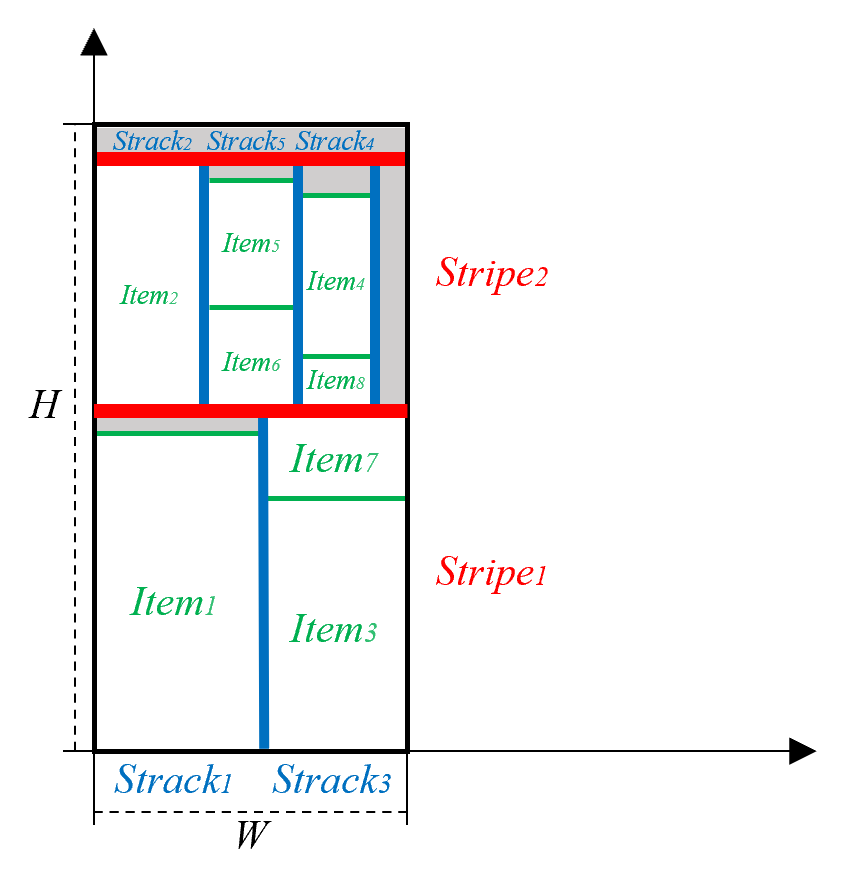
\includegraphics[width=.4\textwidth]{左下角优先排布说明.png}
        \caption{标准排样形式示意图} \label{左下角优先排布说明}
\end{figure}


\textbf{标准排样形式} \quad 对于某一可行解决方案,其使用板材数量及排样方案确定,任一板材中所含产品项的移动并不改变此板材的可利用面积,故不改变整体的板材使用方案及数量。为规范问题分析与求解,通过将每个产品项移动到板材最左边和最下面的位置,形成所谓的排样标准形式,示例见图1。在后续问题讨论中,本文仅考虑标准形式排样。

\subsection{模型建立}

\subsubsection{方向说明}
为便于后续讨论,规定第一阶段切割方向为x方向,即切割方向垂直于高度、平行于长度的方向,如图\ref{方向说明1},与之垂直的板材原片的边的长度规定为板材原片的高度$H$,平行的边的长度规定为板材原片的长度$W$。
\begin{figure}[!htbp]
    \centering
    \begin{minipage}{0.48\linewidth}
        \centering
        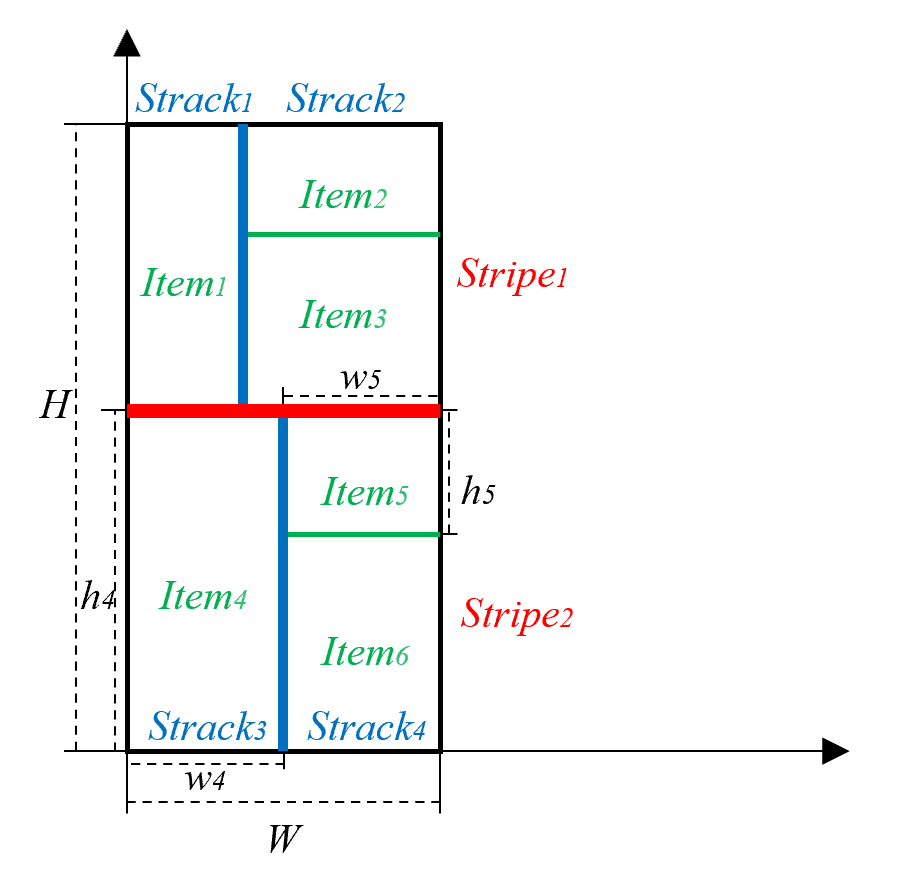
\includegraphics[width=.9\textwidth]{方向说明1.png}
    \end{minipage}
    \begin{minipage}{0.48\linewidth}
        \centering
        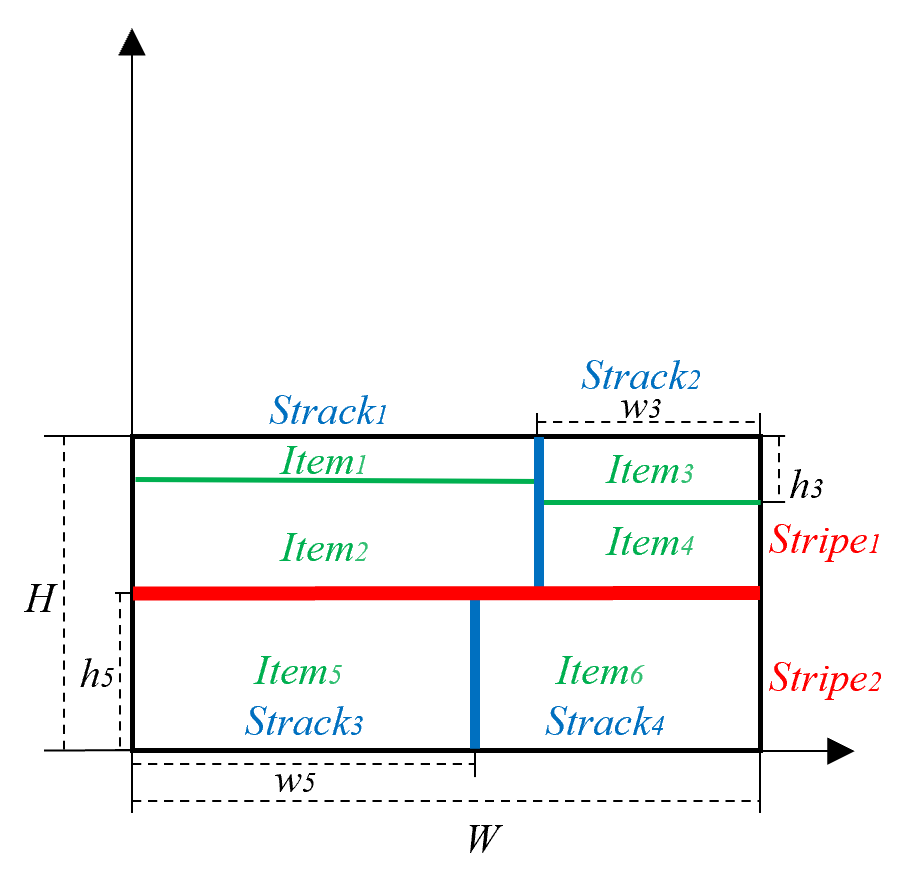
\includegraphics[width=.9\textwidth]{方向说明2.png}
    \end{minipage}
    \caption{原始板材切割示意图}\label{方向说明1}
\end{figure}

\subsubsection{编号规则}
规定按照$h_1 \geq h_2 \geq ...\geq h_n$的顺序,对产品项进行编号。一个可行解决方案最多包含$n$个栈,取栈所含的最高产品项编号作为此栈的编号,也即栈所含所有产品项编号的最小编号。

在此编号规则下,对于栈$j$,可知它一定包含产品项$j$,且产品项$j$为高度最大的项,同时编号小于$j$的产品项均不在此栈中。这种带有包含关系的编号规则,避免了出现重复可行解:即编号不同、但实际所指对象相同,实际为同一可行解的情况。

类似的,一个解决方案最多有$n$个条带,规定用条带所含栈中最高栈对应的编号,作为此条带的编号;一个解决方案最多需要$n$个板材,规定用板材所含条带中最高条带对应的编号,作为此板材的编号。


\subsubsection{模型建立}
在4.2.2节编号规则的约定下,我们定义标志各产品项(Item)、栈(Stack)、条带(Stripe)、板材原片(Bin)之间包含关系的决策变量如下:
\begin{equation}   %\mbox{中文}
    a_{j,i}=
    \begin{cases}
        1, \quad  &  {\rm Item}_i \in   {\rm Stack}_j \\
        0,\quad  &  {\rm Item}_i  \notin   {\rm Stack}_j \\
    \end{cases},\quad j \le n ,\quad j\le i \le n,\quad i,j \in  \mathbb{N}^+  \label{决策变量定义a}
\end{equation}

\begin{equation}
    b_{k,j}=
    \begin{cases}
        1, \quad  &  {\rm Stack}_j \in   {\rm Stripe}_k \\
        0,\quad  &  {\rm Stack}_j  \notin   {\rm Stripe}_k \\
    \end{cases},\quad k \le n ,\quad j\le i \le n,\quad k,j \in  \mathbb{N}^+ \label{决策变量定义b}
\end{equation}

\begin{equation}
    r_{l,k}=
    \begin{cases}
        1, \quad  &  {\rm Stripe}_k \in   {\rm Bin}_l \\
        0,\quad  &  {\rm Stripe}_k  \notin   {\rm Bin}_l \\
    \end{cases},\quad l \le n ,\quad l \le k \le n,\quad l,k \in  \mathbb{N}^+ \label{决策变量定义r}
\end{equation}

在此变量定义下,我们可以计算栈$k$的高度$H(k)$为:
\begin{equation}
    H(k)=\sum_{i=1}^{n} h_i a_{k,i}
\end{equation}


这样引入的模型约束是非线性的,不利于后续的求解。为了获得栈高度的线性表达式,我们引入辅助变量$\delta_{l,i,j}$ ,它表征了产品项$i$对板材$l$中所有条带的高度有影响、并被包含于栈$j$中,其定义如下:
\begin{equation}
    \delta_{l,i,j}=  
    \begin{cases}
        1, \quad  & a_{j,i} r_{l,j}=1\\
        0, \quad  & a_{j,i} r_{l,j}=0
    \end{cases},\quad l \le n-1 ,\quad l+1\le i \le n,\quad l,i \in \mathbb{N}^+ 
\end{equation}
即,$\delta_{l,i,j} = 1$当且仅当项目i包含在栈$j$中,同时栈$j$包含在条带$j$中(则栈i的高度会影响条带$j$的高度),同时条带$j$在板材$l$中。

则我们可以用线性的方式计算板材$l$的已使用高度:
\begin{equation}
\sum_{i=l}^{n} h_i r_{l,i}+\sum_{i=l+1}^{n} h_i \sum_{j=l}^{i-1} \delta_{l,i,j}
\end{equation}

目标函数(\ref{目标函数})是最小化所使用的板材数量,如4.1节中的问题分析,此目标与题意中的尽可能减少板材用量等价,且更为简洁直观、便于计算。当$ r_{l,l}=1 $时表示板材$l$被使用,故(\ref{目标函数})式即为此方案所用的板材总数。
\begin{equation}
    \mathbf{min}  \sum_{l=1}^{n}  r_{l,l} \label{目标函数}
 \end{equation}


根据前述分析,该优化问题涉及变量存在相应约束条件,每个产品项$i$在且仅在一块板材中出现:

\begin{equation}
    \sum_{j=1}^{i}  a_{j,i} =1,\quad \forall i \le n,\quad i \in \mathbb{N}^+ \label{产品项必须排}
\end{equation}


产品项只会被分配给已使用的栈:

\begin{equation}
   \sum_{i=j}^{n}  a_{j,i} \le (n-j+1)a_{j,j},\quad \forall j \le n,\quad j \in \mathbb{N}^+  \label{产品项只给已使用栈}
\end{equation}

排样在同一栈中的产品项必须具有相同的宽度,并且任何一个栈中的产品项的总高度不得超过板材高度$H$:
\begin{equation}
     a_{j,i}=0,\quad \forall j \le n-1,\quad j \in \mathbb{N}^+,\quad  \forall i>j \mid w_i \neq w_j \vee h_i+h_j>H \label{相同宽度}
 \end{equation}

已使用的栈$j$在且仅在一个条带$j$中:
\begin{equation}
    \sum_{k=1}^{n}  b_{k,j} = a_{j,j}, \quad \forall j \le n,\quad j \in \mathbb{N}^+  \label{栈精确排在条带}
\end{equation}

每个栈 $j$的高度不超过所在条带 $k$ 的高度,考虑栈高度可能相同的情况,按照“严格小于”和“小于等于”两张情况予以区分:
\begin{equation}
    \sum_{i=j}^{n} h_ia_{j,i}<\sum_{i=k}^n h_i a_{k,i}+(H+1)(1-b_{k,j}),\quad \forall  2 \le k \le n,\quad \forall j \le k-1, \quad k,j \in \mathbb{N}^+  \label{严格小于的高度限制}
\end{equation}
\begin{equation}
    \sum_{i=j}^{n} h_ia_{j,i} \le \sum_{i=k}^n h_i a_{k,i}+H(1-b_{k,j}), \quad \forall  k \le n-1, \quad \forall k+1 \le j \le n, \quad k,j \in \mathbb{N}^+ \label{小于等于的高度限制}
\end{equation}

条带的宽度不超过箱子的宽度,且栈只会被分配给已使用的条带中:
\begin{equation}
    \sum_{j=1}^{n} w_j b_{k,j} \le W b_{k,k}, \quad k \le n, \quad k \in \mathbb{N}^+ \label{宽度限制}
\end{equation}

每个已使用的条带在且仅在一块板材中:
\begin{equation}
    \sum_{l=1}^{k} r_{l,k} = b_{k,k}, \quad \forall k \le n, \quad k \in \mathbb{N}^+ \label{条带精准打包}
\end{equation}

一块板材上条带的总高度不超过板材的高度:
\begin{equation}
    \sum_{i=l}^{n} h_i r_{l,i} +\sum_{i=l+1}^{n} h_i \sum_{j=l}^{i-1} \delta_{l,i,j} \le H r_{l,l}, \quad \forall l \le n-1, \quad l \in \mathbb{N}^+\label{板材高度}
\end{equation}

根据决策变量的定义式(\ref{决策变量定义a})、式(\ref{决策变量定义r}),设置辅助变量的值:
\begin{equation}
    a_{j,i}+r_{l,j}-1 \le \delta_{l,i,j} \le (a_{j,i}+r_{l,j})/2, \quad \forall l \le n-1,\quad \forall l+1 \le i \le n, \quad l \le j \le i-1, \quad l,i,j \in \mathbb{N}^+ \label{决策变量相关}
\end{equation}

条带只会分配给已使用的板材:
\begin{equation}
    \sum_{k=l+1}^{n} r_{l.k} \le (n-l)r_{l,l}, \quad \forall l \le n-1, \quad l \in \mathbb{N}^+ \label{未使用板材无条带}
\end{equation}

公式(\ref{范围a})-(\ref{范围delta})为变量的范围,所有变量均为0-1整数型变量:
\begin{equation}
    a_{j,i} \in \{0,1\}, \quad j \le n , \quad j \le i \le n, \quad j,i \in \mathbb{N}^+ \label{范围a}
\end{equation}
\begin{equation}
    b_{k,j} \in \{0,1\}, \quad k \le n , \quad j \le n, \quad k,j \in \mathbb{N}^+ \label{范围b}
\end{equation}
\begin{equation}
    r_{l,k} \in \{0,1\}, \quad l \le n , \quad k \le n, \quad l,k \in \mathbb{N}^+ \label{范围r}
\end{equation}
\begin{equation}
    \delta_{l,i,j} \in \{0,1\}, \quad j \le n-1 , \quad l+1 \le i \le n, \quad j,i \in \mathbb{N}^+ \label{范围delta}
\end{equation}

完整的问题一的\textbf{三阶段2BP二进制整数线性规划模型}如下所示:
\begin{equation}
    \begin{cases}
        \mathbf{min}  \sum_{l=1}^{n}  r_{l,l} \\
        s.t.
        \begin{cases}
            \sum_{j=1}^{i}  a_{j,i} =1,\quad i \in \mathbb{N}^+ \\
            \sum_{i=j}^{n}  a_{j,i} \le (n-j+1)a_{j,j},\quad \forall j \le n,\quad j \in \mathbb{N}^+ \\
            a_{j,i}=0, \quad \forall j \le n-1,\quad j \in \mathbb{N}^+,\quad  \forall i>j \mid w_i \neq w_j \vee h_i+h_j>H\\
            \sum_{k=1}^{n}  b_{k,j} =a_{j,j},\quad \forall j \le n,\quad j \in \mathbb{N}^+   \\
            \sum_{i=j}^{n} h_ia_{j,i}<\sum_{i=k}^n h_i a_{k,i}+(H+1)(1-b_{k,j}),\quad \forall  2 \le k \le n,\quad \forall j \le k-1, \quad k,j \in \mathbb{N}^+ \\
            \sum_{i=j}^{n} h_ia_{j,i} \le \sum_{i=k}^n h_i a_{k,i}+H(1-b_{k,j}),\quad \forall  k \le n-1, \quad \forall k+1 \le j \le n, \quad k,j \in \mathbb{N}^+ \\
            \sum_{j=1}^{n} w_j b_{k,j} \le W b_{k,k}, \quad k \le n, \quad k \in \mathbb{N}^+ \\
            \sum_{l=1}^{k} r_{l,k} = b_{k,k}, \quad \forall k \le n, \quad k \in \mathbb{N}^+ \\
            \sum_{i=l}^{n} h_i r_{l,i} +\sum_{i=l+1}^{n} h_i \sum_{j=l}^{i-1} \delta_{l,i,j} \le H r_{l,l}, \quad \forall l \le n-1, \quad l \in \mathbb{N}^+ \\
            a_{j,i}+r_{l,j}-1 \le \delta_{l,i,j} \le (a_{j,i}+r_{l,j})/2, \forall l \le n-1, \forall l+1 \le i \le n, l \le j \le i-1, l,i,j \in \mathbb{N}^+ \\
           \sum_{k=l+1}^{n} r_{l.k} \le (n-l)r_{l,l}, \quad \forall l \le n-1, \quad l \in \mathbb{N}^+ \\
            a_{j,i} \in \{0,1\}, \quad j \le n , \quad j \le i \le n, \quad j,i \in \mathbb{N}^+ \\
            b_{k,j} \in \{0,1\},  \quad k \le n , \quad j \le n, \quad k,j \in \mathbb{N}^+ \\
            r_{l,k} \in \{0,1\}, \quad l \le n , \quad l \le k \le n, \quad l,k \in \mathbb{N}^+ \\
            \delta_{l,i,j} \in \{0,1\},  \quad j \le n-1 , \quad l+1 \le i \le n, \quad j,i \in \mathbb{N}^+
        \end{cases}  \label{问题一模型}
    \end{cases}
\end{equation}


\subsection{模型求解}
	
\subsubsection{数学模型特点分析}

	\textbf{变量多、呈 $ n^2 $ 量级} \quad 所建立的二进制整数线性规划模型,如式子(\ref{范围a})-(\ref{范围delta})所示,其变量个数在 $ n^2 $ 数量级,约束为$ n $的多项式数量级,故随着变量数量增加,求解规模将指数级增长,求解时间长甚至难以在有限步内得到解。 题目所给的数据集基本在 $ 10^3 $ 量级,由此对应的模型规模较大。
	
	\textbf{0-1变量、线性约束} \quad 线性规划求解发展较为成熟,但本模型的变量为0-1二进制整数类型,传统的连续线性规划等方法难以适用。
	

\subsubsection{有限降序首次适应算法(Finite First Fit Decreasing,FFFD)设计}
	
	如4.1节的分析,问题一属于2BP问题,为典型的NP-Hard问题,最优解无法在多项式时间内计算得到。NP-Hard问题有两个求解方向:一是利用传统算法例如分枝定界法、分枝定价算法、动态规划法等,在指数时间内求最优解;二是利用近似算法、近似方案或启发式算法,例如贪心算法、局部搜索、粒子群算法等,在多项式时间内求得近似解。
	
	结合NP-Hard的求解思路与此问题数学模型的特点,提出有限降序首次适应算法(以下简称FFFD算法)进行求解。
	
	\textbf{(1)算法设计}	
	
    \textbf{首次适应算法(First Fit, FF)}	

    首次适应算法(以下简称FF)来源于计算机内存分配问题,FF算法是指当有作业需要内存时,从空闲分区表的第一个表目起查找该表,把最先能够满足要求的空闲区分配给作业。该算法优先利用内存中低址部分的空闲分区,从而保留了高址部分的大空闲区,这为以后到达的大作业分配大的内存空间创造了条件。但是,犹豫低地址不断被划分,容易形成碎片化内存。

    而对于方形件排样问题,FF算法是指将产品项按顺序逐个放在板材上、无法放置在当前板材上时即取出一块新板材,如此放置直至产品项全部放置完成的全过程。FF算法显然可以快速占据原始板材,使得尽可能多的利用板材面积,留出其他原始板材供其他产品项占用。但与内存分配问题类似,FF算法也容易使得原始板材剩余面积碎片化,从而无法达到最优。

    \textbf{有限降序首次适应算法(Finite First Fit Decreasing,FFFD)}	
    
    实际上,与内存分配问题不同,方形件排样问题中,可以提前已知所有产品项的形状与大小。因此在进行FF算法运算前,提前对产品项进行排序则是一种避免原始板材剩余面积碎片化的方法。在该问题中,可以将产品项降序排列,进而完成方形件的排样优化问题,该方法即成为有限降序首次适应算法。在本文中,规定对产品排序时使用高度优先原则,在将产品项排入原始板材时,使用左下优先(Bottom-Left,BL)原则。

    该FFFD算法可以描述为采用高度降序的顺序将产品项放入有序表中,只要产品项有序表不为空,算法会一个一个将产品项排进板材中。放置判断思路为:产品项的栈会尽可能长的添加到当前条带中,若当前条带无法再放进任何产品项,则会在当前板材中新增一个空条带,如果没有产品项能放入此新的空条带,则丢弃此空条带,将此板材添加进解决方案,并初始化新板材。

    \textbf{(2)算法最优性证明 }	
	
	文献\cite{FFFD}已证明,用降序首次拟合方法解决二维装箱问题,在最坏情况下得到最优解的概率为22\%,而在实际中,该方案通常比22\%的界限更接近最优,故仅需一些简单的经验法则,就可以得到近似最优解。
	
	
	针对方形件排样问题所提出的FFFD算法,是在首次拟合原则的基础上,加上了产品项降序排序及有限次步骤限制,因此理论上FFFD算法可以得到问题的最优解。

	% \textbf{从实际生产角度出发}	
	
	% 从结果上看,排样优化问题一是一个产品项如何布局,使得耗材最少的静态排样问题。而实际生产工作中,实现方形件的排样、切割是一个动态的过程。故从动态实现排样动作的角度,可将该问题转化为:存在某种最优的顺序,使得若将产品项按此顺序逐个放在板材上、无法放置在当前板材上时即取出一块新板材,如此放置直至产品项全部放置完成的全过程,能够满足切割条件,并使得板材总用量比其它顺序放置最少。
	
	% FFFD算法旨在从动态视角模拟方形件排样过程,以某种顺序逐个完成产品项在板材上的放置,使得总板材量最少。理论上若FFFD算法的产品项排序为前述最优顺序,就可以得到最优解。
	
	% \textbf{产品项排序顺序选择}		
	
	% 从理论上分析,考虑实际排样场景,宽度近似的情况下,高度较长的产品项相比高度较短的产品项,对板材余料的可用性要求更高,即能找到可容纳的板材类型更少。因此优先考虑高度更长的产品项纳入板材排样,由高度小的板材作为灵活插入项,去提高已排长产品项的各板材的使用面积,理论上可一定程度上比随机选取产品项排样效率更好。从实际测试上分析,经多种不同顺序排序的测试,降序排序整体表现最优,故选取此顺序合理。
	
	% 由此,FFFD算法采用高度降序的顺序将产品项放入有序表中,只要产品项有序表不为空,算法会一个一个将产品项排进板材中。放置判断思路为:产品项的栈会尽可能长的添加到当前条带中,若当前条带无法再放进任何产品项,则会在当前板材中新增一个空条带,如果没有产品项能放入此新的空条带,则丢弃此空条带,将此板材添加进解决方案,并初始化新板材。
	
	\subsubsection{FFFD算法步骤}	
	
	FFFD算法的具体执行逻辑为:
	
	1)对所有的产品项,按照高度降序排序,放入待排样产品项有序表(以下简称有序表)里;
	
	2)当有序表非空时,创建一个新的板材B,若有序表已空则跳至步骤6)结束程序;
	
	3)创建一个新的条带记为S,初始化其宽为板材宽度$W$,高为0,所含栈为空。遍历有序表,记当前产品项为I:
	
	a. 如果S为空,且I可以放进其中,则放入,并将I从有序表中移去、更新S信息;
	
	b. 如果S非空,且I可以放进其中,则放入,并将当前I从有序表中移去、更新条带,然后遍历有序表中的剩余项记为$\rm{I}_2$,若$\rm{I}_2$放入I所在栈的,则将$\rm{I}_2$放入此栈,并将$\rm{I}_2$从有序表中移去、更新S信息;
	
	(其中,当条带为空时,产品项能放进此条带的判据是:产品项的宽度小于条带的未使用宽度,且高度小于板材的未使用高度。当条带不为空时,产品项能排进此条带的判据是:当前产品项的宽度小于条带的未使用宽度,且高度小于条带的未使用高度。产品项2能放入某一产品项所在栈的判据是:两个产品项的宽度相同,且产品项2的高度小于此栈所在条带的未使用高度)
	
	4)如果S不为空,则重复步骤3)至 步骤4);
	
	5)如果S为空,丢弃此空S,将此B添加进可行解方案中,跳至步骤2);
	
	6)结束程序,此时有序表为空,得到一个包含一定数量板材及每个板材上排样的产品项信息的可行解方案。

	另外,考虑\textbf{产品项的可旋转性},即宽度和高度并没有硬性的大小限定,方形件在板材上可旋转90°、宽度和高度的值对换,则在算法步骤1)的产品有序表生成时,将原有产品项复制增加一份并加入到有序表中,复制项与原项的宽度、长度对换,并使当某产品项从有序表中移出时,其宽高对换的相应项也移出有序表,保证实际所得排样结果产品项的唯一性。

\subsection{启发式算法}	

对于该大规模混合整数模型,还可以进一步使用启发式算法求解,由于模型规模巨大,一个良好的初值对于提高启发式算法收敛速度起着重要作用。而FFFD刚好可以给启发式算法提供良好的初值。

本文在FFFD的基础上,采用遗传算法、离散二进制粒子群算法对排样优化策略进一步优化。在此问题中,将$a_{j,i}$,$b_{k,j}$,$c_{l,k}$,$\delta_{l,i,j}$串联起来,即可形成一维二进制向量,进而作为遗传算法和离散二进制粒子群算法的求解初值。对于遗传算法、离散二进制粒子群算法的其他初值,也可以在将产品项顺序$\text{Item}$随机打乱后,再通过有限首次适应(Finite First Fit)算法得到排样优化问题可行解,并形成靠近优化问题全局最优解的可行解初值。

在遗传算法和离散二进制粒子群算法中,原规划问题的约束通过罚函数的方式加入到优化目标,即新的优化目标为:
\begin{equation}
    obj = \sum_{l=1}^{n}  r_{l,l} + k\sqrt{k}h(x), l \le n,l \in \mathbb{N}^+\label{启发式算法}
\end{equation}
\noindent 式中,$k$表示遗传算法或离散二进制粒子群算法当前迭代次数,$x$表示所有决策变量,$h(x)$表示在变量$x$下所谓反的约束的总和。

于是,在式\ref{启发式算法}下,排样策略可以进一步进行迭代优化。

\subsection{求解结果}

	运行FFFD算法对数据集A进行求解,800个左右产品项数量的数据集,200ms左右即可计算完毕,得到结果如表1所示。
    
    \begin{table}[htph]
        \centering
        \caption{问题一 FFFD算法求解结果}
         \label{问题一 FFFD算法求解结果}
        \begin{tabular}{ccccc}
         \hline
         \makebox[0.2\textwidth][c]{数据集}&\makebox[0.16\textwidth][c]{A1}&\makebox[0.16\textwidth][c]{A2}&\makebox[0.16\textwidth][c]{A3}&\makebox[0.16\textwidth][c]{A4}\\ \hline
         利用率 &0.94933&0.93117& 0.95147&0.94083 \\ \hline
         产品项总数&752&731&823&799 \\ \hline
         板材数&88&89&88&87\\ \hline
         FFFD求解耗时(ms)&188.49&172.47&214.30 &201.28 \\ \hline 
        \multicolumn{5}{l}{【注】:板材利用率 = 产品项面积之和 / 使用原片面积之和}\\
        \end{tabular}
        \end{table}
	
        数据集A1-A4部分板材的排样方案效果图如图3-6所示,其余排样方案效果图详见附录。
        \begin{figure}[!htbp]
            \centering
            \begin{minipage}{0.48\linewidth}
                \centering
                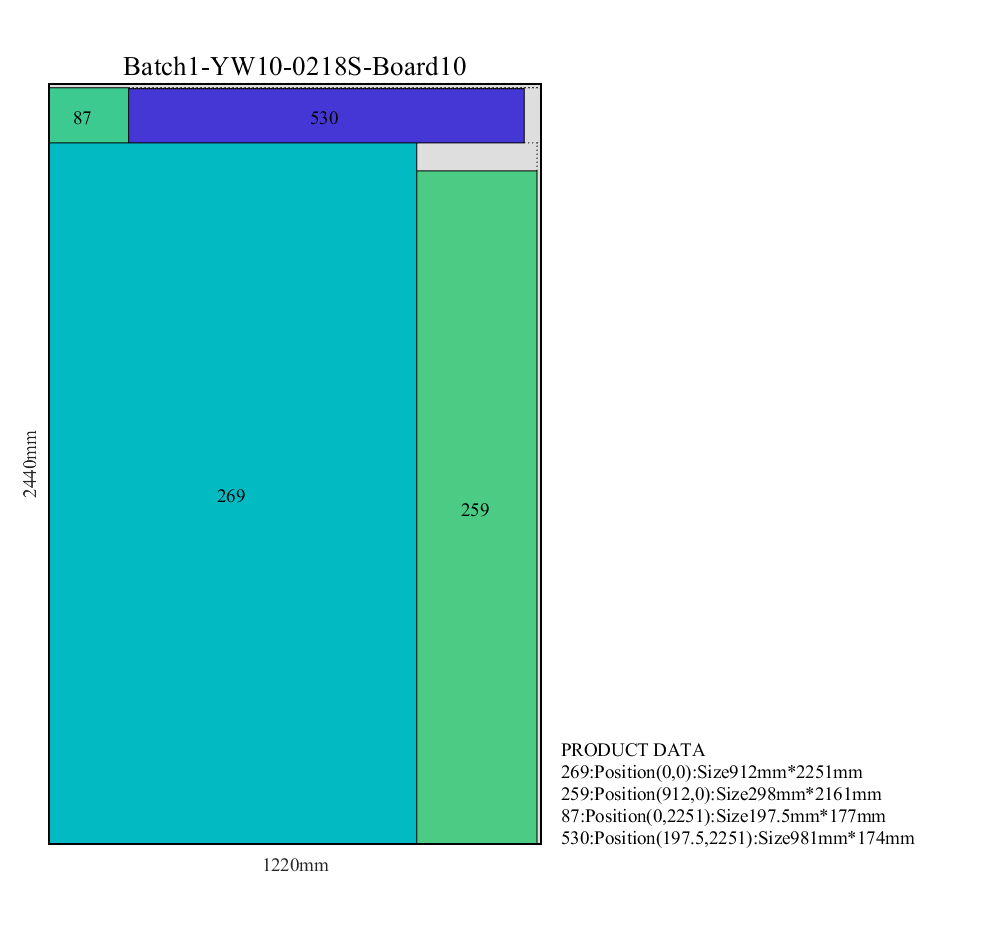
\includegraphics[width=.9\textwidth]{A1-Batch1-YW10-0218S-Board10.png}
                \caption{数据集A1(板材10)}
            \end{minipage}
            \begin{minipage}{0.48\linewidth}
                \centering
                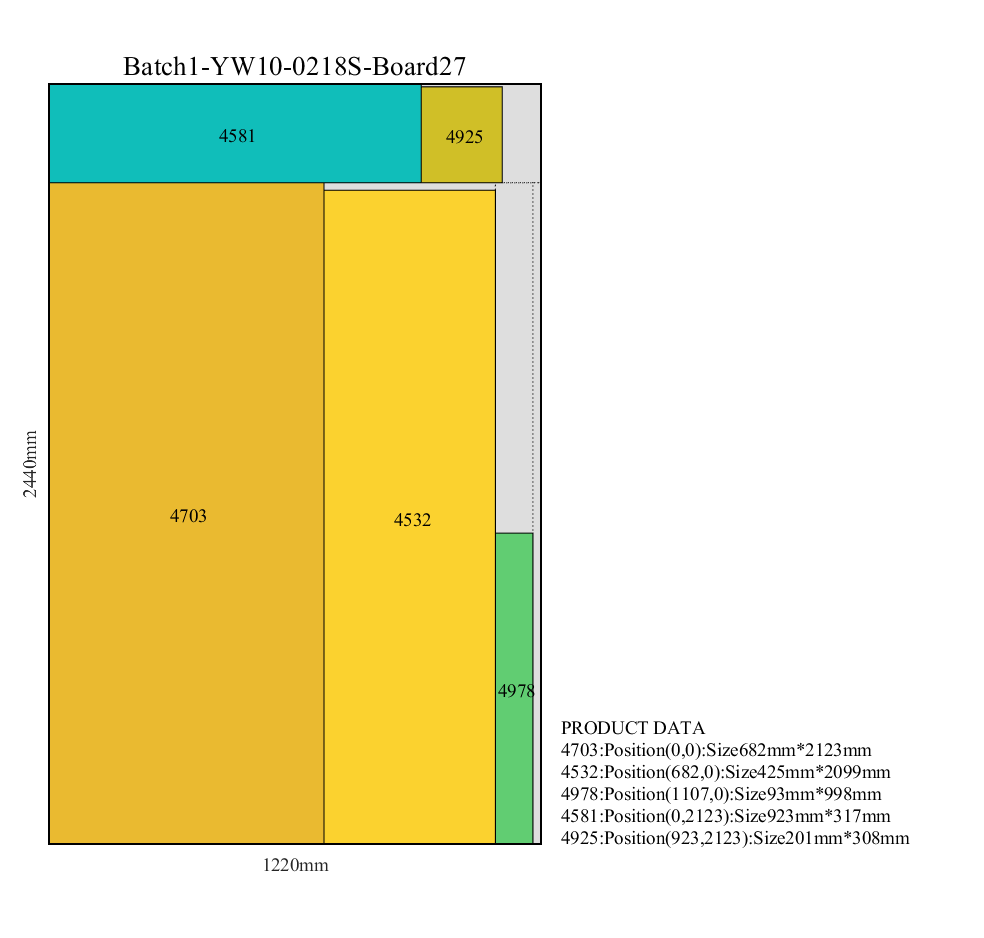
\includegraphics[width=.9\textwidth]{A2-Batch1-YW10-0218S-Board27.png}
                \caption{数据集A2(板材27)}
            \end{minipage}
        \end{figure}
        \begin{figure}[!htbp]
            \centering
            \begin{minipage}{0.48\linewidth}
                \centering
                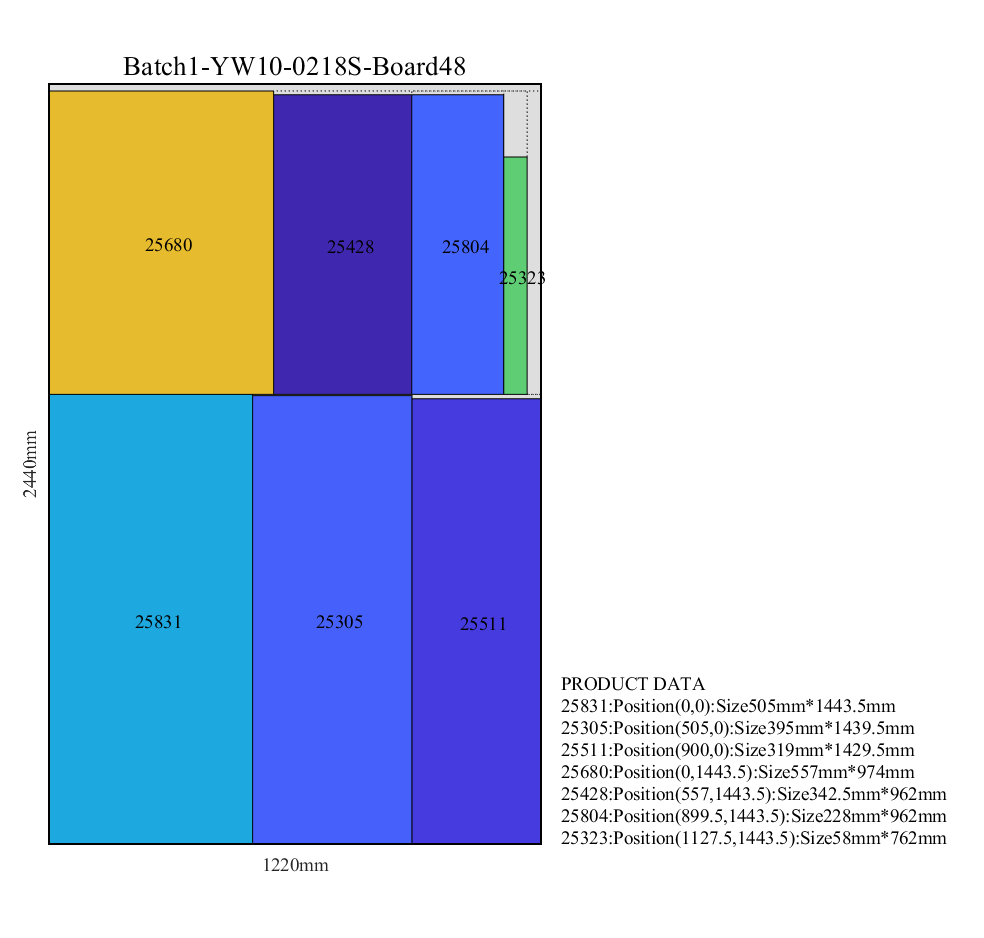
\includegraphics[width=.9\textwidth]{A3-Batch1-YW10-0218S-Board48.png}
                \caption{数据集A3(板材48)}
            \end{minipage}
            \begin{minipage}{0.48\linewidth}
                \centering
                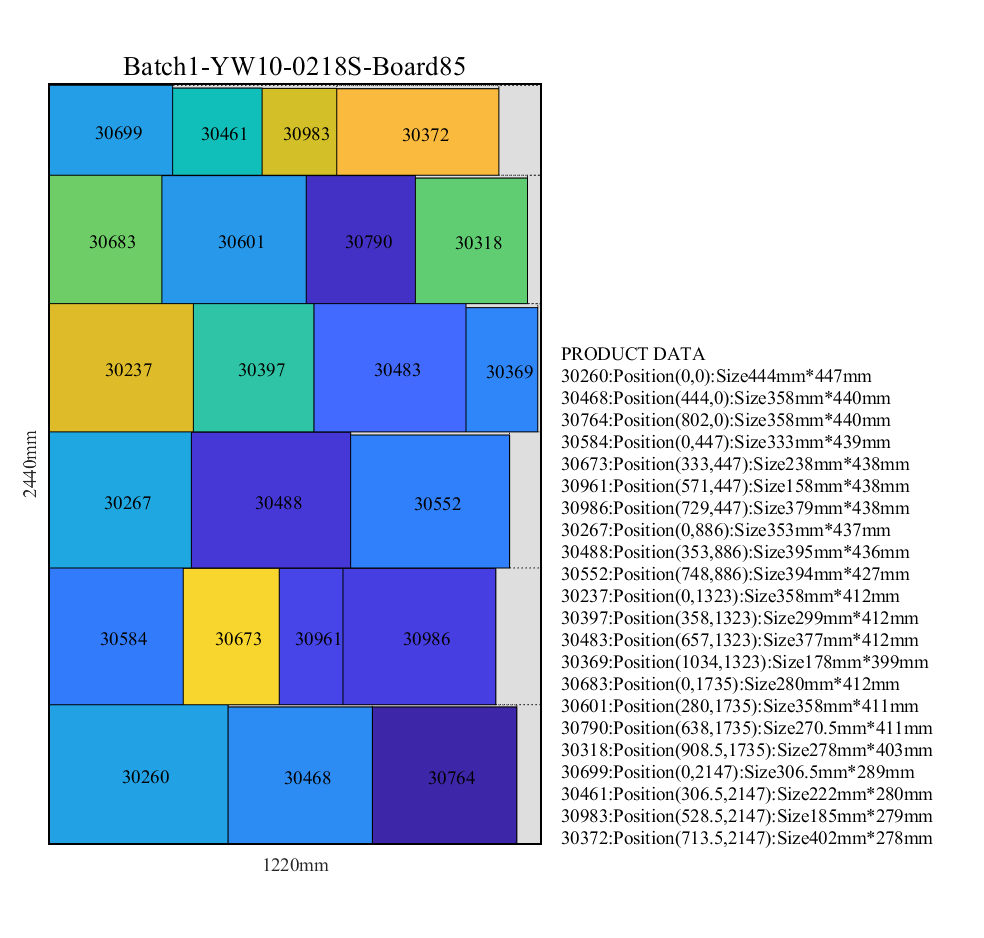
\includegraphics[width=.9\textwidth]{A4-Batch1-YW10-0218S-Board85.png}
                \caption{数据集A4(板材85)}
            \end{minipage}
        \end{figure}
	

\subsection{算法及效果评价}

\subsubsection{复杂度指标评价}  

经计算,FFFD算法程序空间复杂度为$O(n)$,最好时间复杂度为$O(n)$,最坏时间复杂度为 $ O(n^2) $。FFFD算法为有限实现算法,表现为算法在有限步骤内可求得解。该算法逻辑简单,复杂度低,计算效果好,而启发式算法求解速度慢,求解效果也并不优于该FFFD算法.因此,在实际应用中,FFFD算法作为方形件排料优化的计算方法。


\subsubsection{求解有效性}
	
	以数据集dataA1为例,由FFFD算法求得的板材数为88,与以下两个数据对比:
	
	\textbf{理想最少值} \quad 假定原始板材可以随意切割、拼接的情况下,即此时所需原始板材的数量仅和原始板材与产品项的形状无关。 所有产品项的面积和为 $ S_{items} = 248685614.55 mm^2 $,若可以随意切割、拼接,则需要的板材数为: $ S_{items}/H/W =  83.54 $
	
	\textbf{商用排样软件} \quad 将板材原件规格和数据集A1的产品项信息输入某商用专业板材优化软件,得到不考虑三阶段一刀切约束下的最优板材数为86
	
	而问题一相比上述两个场景,多了严格的切割约束,FFFD算法求得的结果仅多个别板材数,由此可见,FFFD算法具有较好的求解有效性。

	
\subsubsection{运行时间}
	 
	数据集A1-A4的产品项规模在800片左右,FFFD算法求解平均耗时在200毫秒左右,求解效果好,运行时间快。
    
    启发式算法因其并未得到更优于FFFD的解,所以此处不再记录其运行时间。
		


\section{问题二订单组批}

\subsection{问题分析}
该问题中要求订单当且仅当出现在一个批次中,即订单不可拆分,所以该问题也可简述为在问题一的基础上完成订单的组合问题。这仍然是一个NP-Hard问题,若简单沿用问题一的混合整数线性规划模型(\ref{问题一模型}),引入新的变量与约束,这会使得模型求解难度进一步增大,求解时间增长,显然这并非是解决该问题合适的方法。

因此,本问题将在问题一的基础上,进一步建立\textbf{两步优化模型},内层模型求解最优排样方案,外层模型求解最优组批方案,显然这是一个带有线性约束及非线性目标函数的混合整数非线性规划问题。

\subsection{模型建立}


\subsubsection{决策变量}

类似问题一中(\ref{决策变量定义a})、(\ref{决策变量定义b})、(\ref{决策变量定义r})的变量定义方法,定义批次的编号为该批次所包含的最小的订单编号,则有描述各批次(Batch)、订单(Order)之间包含关系的决策变量如下:
\begin{equation}   %\mbox{中文}
    d_{q,p}=
    \begin{cases}
        1, \quad  & \text{Order}_p \in  \text{Batch}_q \\
        0,\quad  & \text{Order}_p \notin  \text{Batch}_q \\
    \end{cases},\quad q\le p \le m,\quad p,q \in  \mathbb{N}^+\\
\end{equation}
\noindent 式中,$m$为订单总数。


\subsubsection{模型建立}
该问题目标函数为总的板材利用率最高,为总原始板材使用数量最少。

\textbf{定义}非线性函数$f_q(d_{q,1},d_{q,2},\cdots,d_{q,m})$,表示在第$q$批次的订单组合$(d_{q,1},d_{q,2},\cdots,d_{q,m})$利用问题一模型所求得的最佳排样方案所使用的原始板材数量。

即有非线性目标函数
\begin{equation}   
    \mathbf{min}\quad\sum_{q=1}^{m} f_q(d_{q,1},d_{q,2},\cdots,d_{q,m}),q\le m ,q\in  \mathbb{N}^+\label{目标函数2}
\end{equation}

该目标函数中,函数$f_q$可利用问题一模型求解,函数$f_q$的优化求解问题,即为该组批优化的内层优化问题。

为保证所有的订单$p$被批次$q$包含且仅包含1次,有

\begin{equation}   
    \sum_{q=1}^{p} d_{q,p}=1,\quad \forall p\le m,p \in \mathbb{N}^+ \label{订单必须排} 
\end{equation}


在$d_{q,p}$的编号原则约定下,需要保证订单$p$仅分配给非空的批次$q$,故有

\begin{equation}   
\sum_{p=q}^{m} d_{q,p} \le (m-q+1)d_{q,q},\quad \forall q\le m,q\in \mathbb{N}^+\label{编号原则2}
\end{equation}

定义$N_p$为订单p所包含的产品项个数,为保证加工环节快速流转,每个批次产品项总数不能超过限定值,则有

\begin{equation}   
    \sum_{p=q}^{m} N_pd_{q,p} \le \text{max\_item\_num},\quad \forall q \le m, q\in \mathbb{N}^+
\end{equation}

定义$S_p$为订单p所包含的产品项总面积,因工厂产能限制,每个批次产品项的面积总和不能超过限定值,所以有

\begin{equation}   
    \sum_{p=q}^{m} S_pd_{q,p} \le \text{max\_item\_area},\quad \forall q\le m,q\in \mathbb{N}^+
\end{equation}

决策变量的取值范围:
\begin{equation}
    d_{q,p} \in \{0,1\},  \forall p,q,\quad,q\le p \le m,  p,q\in \mathbb{N}^+
\end{equation}

因此,可以得到混合整数非线性规划模型
\begin{equation}
    \begin{cases}
        \mathbf{min} \sum_{q=1}^{m} f_q(d_{q,1},d_{q,2},\cdots,d_{q,m}) \\
        \mathbf{s.t.}
        \begin{cases}
            \sum_{q=1}^{p} d_{q,p}=1,\quad \forall p\le m,p \in \mathbb{N}^+ \\
            \sum_{p=q}^{m} d_{q,p} \le (m-q+1)d_{q,q},\quad \forall q\le m,q\in \mathbb{N}^+  \\
            \sum_{p=q}^{m} n_pd_{q,p} \le \text{max\_item\_num},\quad \forall q \le m, q\in \mathbb{N}^+\\
            \sum_{p=q}^{m} S_pd_{q,p} le max\_item\_area,\quad \forall q\le m,q\in \mathbb{N}^+ \\
            d_{q,p} \in \{0,1\}, \forall p,q,\quad,q\le p \le m,  p,q\in \mathbb{N}^+\\
        \end{cases}  \label{问题二模型}
    \end{cases}
\end{equation}


\subsection{模型求解}
\subsubsection{数学模型特点分析}
	\textbf{数学模型特点} \quad 该数学模型外层模型为混合整数非线性模型,与问题一类似,该数学模型仍然具有变量多、量级重的问题,变量数量呈 $ n^2 $ 量级。此外,由于该模型为两步优化模型,所以内层模型的优化速度也极大程度的影响了整个模型的迭代求解过程。
	
	\textbf{内层模型求解} \quad 由于内层模型的计算速度和准确性极大程度的影响了全局模型的优化效率和效果,所以综合考虑此处内层模型使用问题一4.3.2节中FFFD算法求解。
	
	\textbf{外层模型求解} \quad 传统算法仍难以解决该类大规模混合整数非线性规划问题,设计合适的贪心算法并求得该模型的局部最优解,仍然是求解该模型的关键。

\subsubsection{优先搜索算法(First Search, FS)设计}
该算法旨在解决订单组批问题,为了后文更好的描述求解算法,将该问题做如下描述:现总共有$m$个生产批次,每个生产批次仅含1个订单,通过合适的方法,将多个批次组合为1个批次,从而降低板材使用数量,提高板材利用率。

在解决该一般问题之前,先考虑一组特异性数据。

\textbf{特异性问题}

1)假定在所有产品项中材质$t$的产品项有且仅有2个,分别被2个批次$\text{Batch}_1$、$\text{Batch}_2$包含,且两个产品项可排样在1块原始板材上。

显然,当且仅当这2个批次被组合到一起时,该材质所使用的原始板材数量才会减少。否则,该材质的板材利用率不会再提高。

2)相反地,对于产品项数量更多的材质$t'$,其被批次$q'$等多个批次所包含。

此时,如若因为约束等因素限制,使得这些批次中两个或几个批次不能再次与批次$q'$组合。但是仍然可能会有其他可选批次与订单$p'$组合,并提高其板材利用率。而且由于其产品项数量多、形状多,在排样时可选方案也更多,该类材质往往能有较高的板材利用率。

因此,在此种情况下,情况1)中的订单组合到同一个批次中带来的收益往往会大于情况2)中的订单组合。换言之,在组合订单时,情况1)中的订单可以优先考虑。

\textbf{一般问题}

基于以上讨论,可以得出经验性结论,即当材质$t$的产品项被尽可能的少的批次所包含、且材质$t$的产品项能够被排样到尽可能的少的原始板材时,包含材质$t$的产品项的批次在组合时应有更高的优先级。

因此,为解决该一般问题,可以将合并后能够产生收益(使得该类材质使用的原始板材数量减少,例如特异性问题中的情况1))且满足题目约束的两个此类批次优先整合到一起。组合后,这两个批次转换为一个批次,于是,该问题再次转变为批次组合问题,可以继续以相同的方式,对剩下的批次进行组合,直到剩下的批次中任意两个组合在一起都不能继续提高板材利用率。



\subsubsection{优先搜索算法步骤}

1) 初始化订单$p$的生产批次为第$q$($q=p$)批。

2) 对每种材质全部产品项进行排样,并按照包含该种材质的批次数量升序排列,当包含该种材质的批次数量一致时,按照该种材质全部产品项排样所需的原始板材的数量升序排列。排在前位的材质中的批次,具有更高的组合优先级。

3) 按照第2)步形成的材质顺序进行搜索,对于材质t,如果包含材质t的批次不少于2个,则考虑其任意2个批次合并后,是否可以有效的减少该材质t的原始板材使用数量。

4) 如果可以减少该材质t的原始板材使用数量,同时2个批次合并后不违反单个批次产品项综述约束及面积总和约束,则将该2个批次合并,回到步骤2) 重新排样并排序。否则,回到步骤3) 继续搜索下一材质。

5) 当全部材质搜索结束,这说明此时任何两个批次合并到一起,都不会再减少总的板材使用数量,即无法进一步提高板材利用率。此时,得到订单组批方案。

6) 对不连续的批次编号重新整理、编号,输出求解结果。

7) 此时的订单组批方案中,并非所有批次都接近单个批次产品项总数上限或面积总和上限,其小规模的批次仍完成可进一步合并,以减少批次数量。然而,考虑到此种合并不会进一步提高板材利用率,与本文的优化目标无关,且这种组合方法可以较易实现,因此,本文不再考虑对批次的进一步合并的问题。

% 算法\ref{test}
% \begin{algorithm}
%     % \SetAlgoNoLine
%     \caption{Put your caption here}\label{test}
%     \begin{multicols}{2}
%         \SetAlgoLined
%         \KwData{this text}
%         KwResult{how to write algorithm with \LaTeX2e }
%         initialization\;
%         \While{not at end of this document}{read current\;
%         \eIf{understand}
%         {go to next section\;current section becomes this one\;
%         }{
%         go back to the beginning of current section\;
%         }
%         }
%     \end{multicols}
% \end{algorithm}

\subsection{求解结果}

	运行算法对数据集B进行求解,所得结果如表\ref{问题二 优化搜索算法求解结果}所示。
    \begin{table}[htph]
        \centering
        \caption{问题二 优化搜索算法求解结果}
         \label{问题二 优化搜索算法求解结果}
        \begin{tabular}{cccccc}
         \hline
         \makebox[0.2\textwidth][c]{数据集}&\makebox[0.12\textwidth][c]{B1}&\makebox[0.12\textwidth][c]{B2}&\makebox[0.12\textwidth][c]{B3}&\makebox[0.12\textwidth][c]{B4}&\makebox[0.12\textwidth][c]{B5}\\ \hline
         利用率&0.79231&0.77665&0.77942& 0.78172&0.76591 \\ \hline
	     批次数&44&35&34&35&45 \\ \hline
         板材总数&3759&2481&2620&2597&4034 \\ \hline
         求解耗时(s)&0&0&0&0&0\\ \hline
         
        \end{tabular}
    \end{table}

    所得利用率在 76\%至80\% 之间,相比问题一较低,这主要由于同一订单的产品项必须在相同批次,而材质不同的产品项无法排样在同一块板材原件上所导致。由输出结果所得各组批的排样图分析可见,在此组批约束下,此排样结果已相对较优。各组批方案详见附录。

    \begin{figure}[!htbp]
        \centering
        \begin{minipage}{0.48\linewidth}
            \centering
            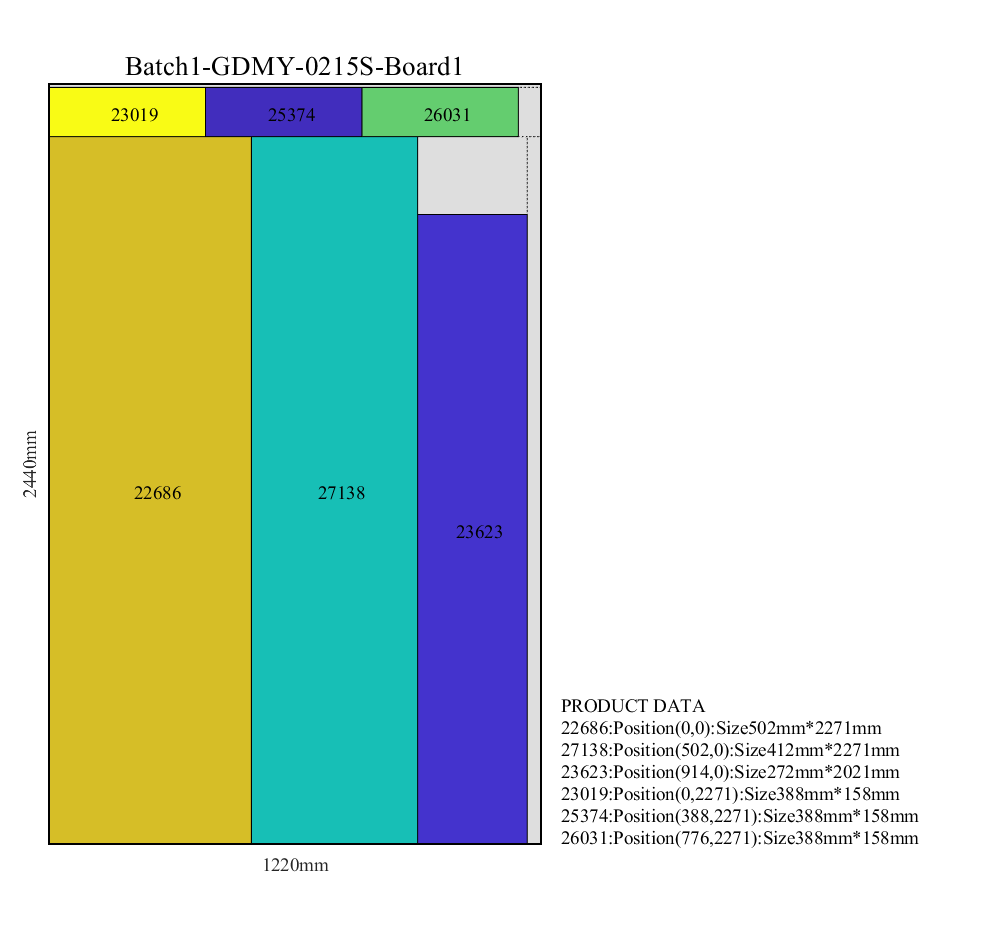
\includegraphics[width=.9\textwidth]{B1-Batch1-GDMY-0215S-Board1.png}
            \caption{数据集B1(批次1板材1)}
        \end{minipage}
        \begin{minipage}{0.48\linewidth}
            \centering
            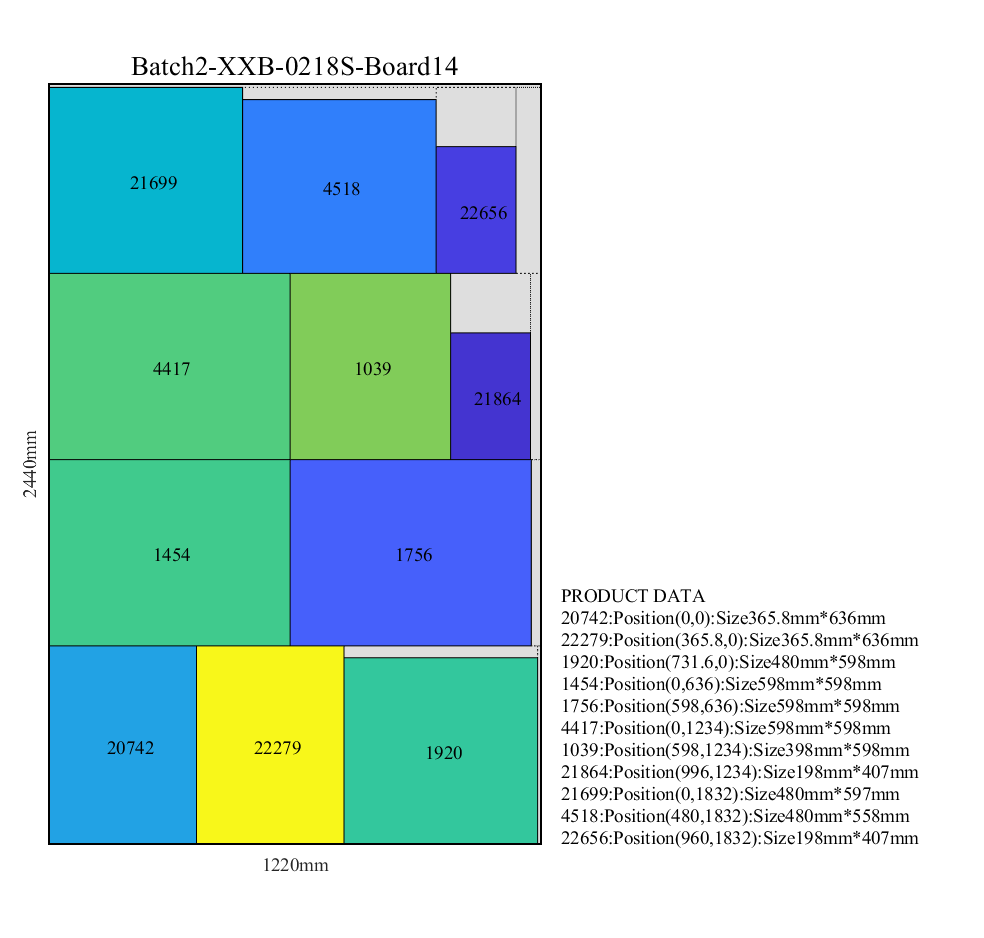
\includegraphics[width=.9\textwidth]{B2-Batch2-XXB-0218S-Board14.png}
            \caption{数据集B2(批次2板材14)}
        \end{minipage}
    \end{figure}
    \begin{figure}[!htbp]
        \centering
        \begin{minipage}{0.48\linewidth}
            \centering
            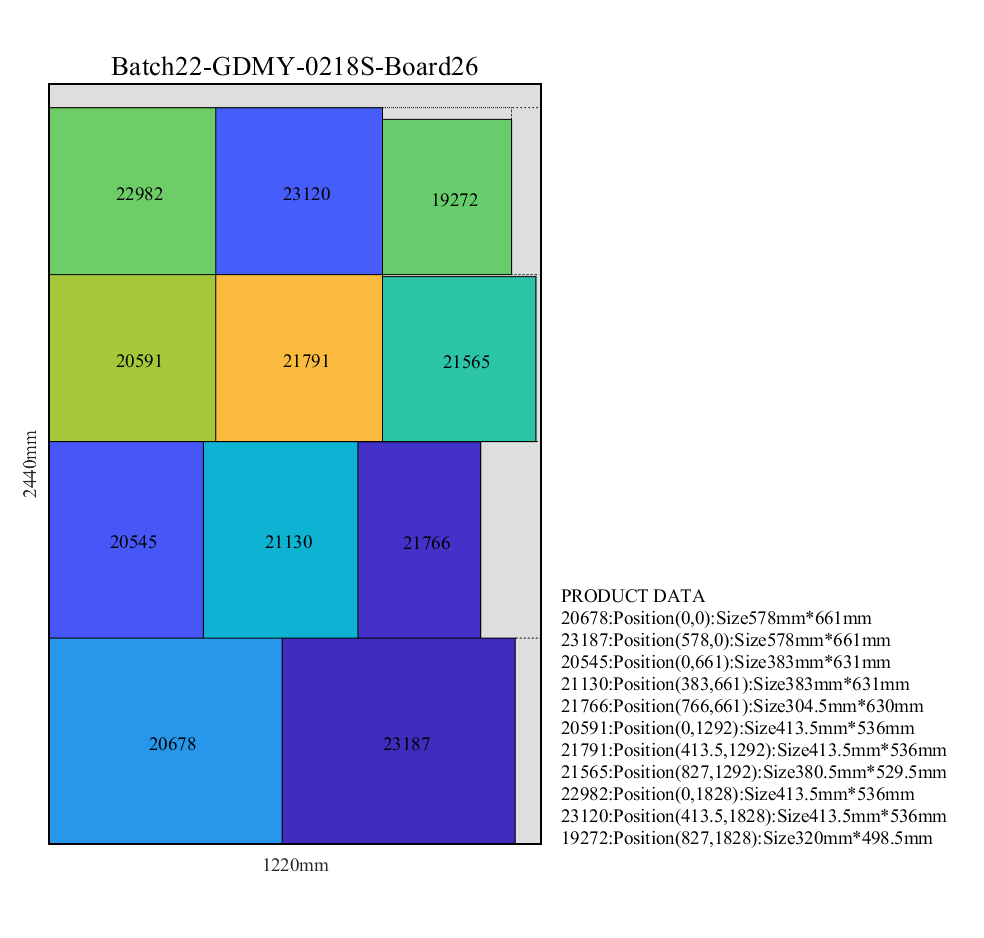
\includegraphics[width=.9\textwidth]{B3-Batch22-GDMY-0218S-Board26.png}
            \caption{数据集B3(批次22板材26)}
        \end{minipage}
        \begin{minipage}{0.48\linewidth}
            \centering
            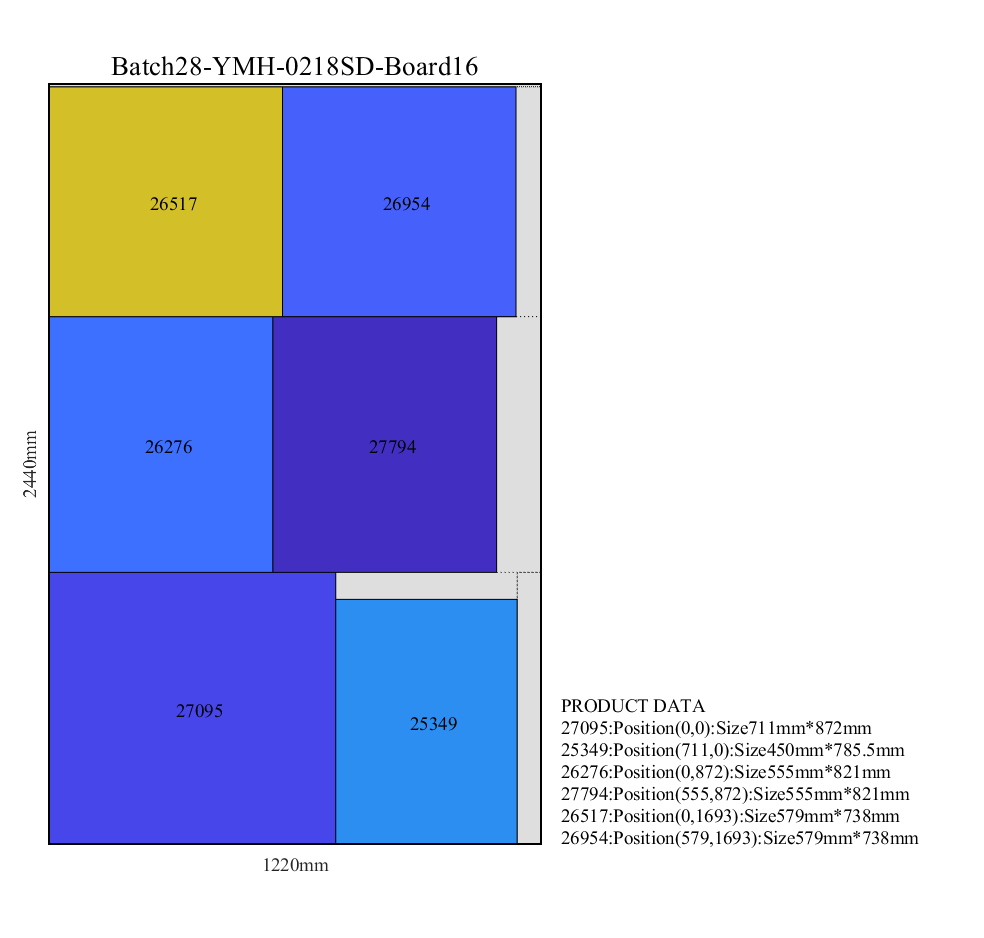
\includegraphics[width=.9\textwidth]{B4-Batch28-YMH-0218SD-Board16.png}
            \caption{数据集B4(批次28板材16)}
        \end{minipage}
        \begin{minipage}{0.48\linewidth}
            \centering
            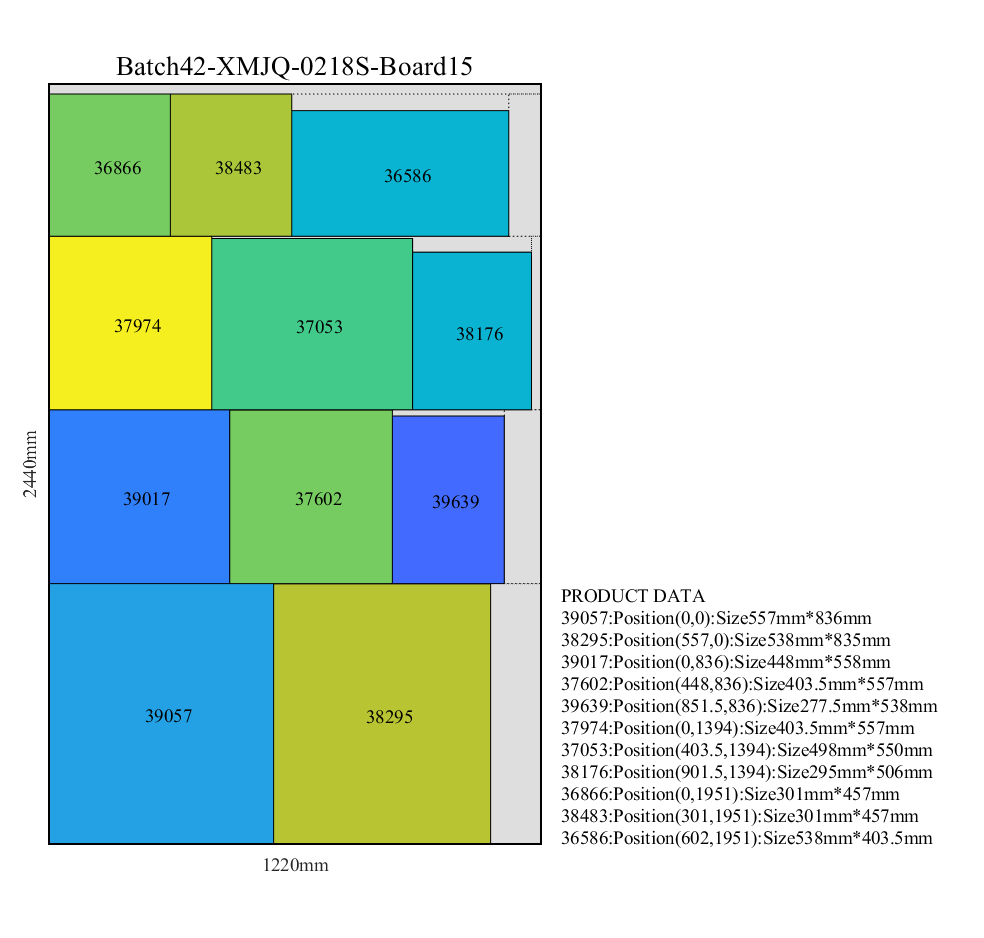
\includegraphics[width=.9\textwidth]{B5-Batch42-XMJQ-0218S-Board15.png}
            \caption{数据集B5(批次42板材15)}
        \end{minipage}
    \end{figure}

\subsection{算法及效果评价}

% \subsubsection{复杂度指标评价}  

% 经计算,优先搜索算法程序空间复杂度为$O(n)$,最好时间复杂度为$O(n)$,最坏时间复杂度为 $ O(n^2) $。FFFD算法为有限实现算法,表现为算法在有限步骤内可求得解。该算法逻辑简单,复杂度低,计算效果好,因此,在实际应用中,FFFD算法作为方形件排料优化的计算方法。

	
\subsubsection{运行时间}
	 
	数据集B1-B5的产品项规模在20000-30000片左右,算法求解平均耗时在20min左右。对于该大规模深度耦合复杂程度问题,此求解时间速度快,效果好。
		
\subsubsection{求解有效性}

以数据集dataB1为例,由优先搜索算法求得的板材数为3759片,与以下理想数据对比:

\textbf{理想最少值} \quad 假定原始板材可以随意切割、拼接的情况下,即此时所需原始板材的数量仅和原始板材与产品项的形状无关,仅与面积有关。此时,将所有产品放入同一个批次,按照每个材质所有产品项的面积和$S_t$,与原始板材的面积$S_0$对比,得到在可以随意切割、拼接的情况下,需要的板材数为3051片。

\textbf{忽略数量及面积约束} \quad 忽略产品项数量及面积约束,将所有产品放入同一个批次,同时加工,利用问题一FFFD方法对此批材料排样,可得此时最优排样方案需要原始板材3335片。


而问题二相比上述两个场景,多了严格的切割约束或产品项数量及面积约束,FFFD算法求得的结果仅增加少量原始板材数,由此可见,优先搜索算法的求解有效性。



\section{模型评价与展望}
\subsection{模型优点}
\begin{itemize}
    \item 排样优化与组批优化算法计算时间较快,排样优化求解800规模产品项仅需200ms左右,组批优化求解30000规模产品项仅需20min左右;
    \item 排样优化与组批优化算法计算效果较优,使得最小原始板材数量接近于理想值;
    \item 排样考虑了方形件的旋转问题,对产品项的宽度和高度没有绝对的大小关系限制,允许产品项以旋转或不旋转的方式排样在板材中,可行解空间更大。
\end{itemize}
\subsection{模型缺点}
\begin{itemize}
    \item 原大规模混合整数线性规划问题变量及约束数量多,难以用常规方法直接求解;
    \item 排样优化中采用产品项高度作为降序排序,可能存在其他顺序甚至不同级循环的复合排序表现更优,需要进一步论证与测验;
    \item 组批优化中未考虑小规模生产批次的进一步合并,在实际生产中多个小规模生产批次可能导致人工、设备运行等成本高、仓储容量利用率低、边际收益较小等问题。
\end{itemize}

\subsection{未来展望}
\begin{itemize}
	\item 通过寻找变量之间的隐含约束关系、在求解过程中判断并舍弃不可能存在的变量值等方式,降低混合整数线性规划模型的规模,加快模型求解;
	\item FFFD算法对顺序敏感,不同应用场景或不同的数据集,理论最优顺序会有所不同,可以根据输入数据集的不同,对数据集进行预先训练、特性辨识等,寻找适合于不同数据集的各异排序,使算法具有自适应性;
	\item 输入更多的约束例如仓储容量使用率、最低产品项生产数等,对组批优化产生的多项小规模生产批次做进一步的组合,使组批算法的实际使用价值更高。
\end{itemize}



\newpage
\quad
\newpage

%参考文献   手工录入
%\begin{thebibliography}{9}%宽度9
% \bib {\rm Item}{bib:one} ....
% \bib {\rm Item}{bib:two} ....
%\end{thebibliography}

%采用bibtex方案
\bibliographystyle{gmcm}
\bibliography{MCM_2022}

\cite{mittelbach_latex_2004,wright_latex3_2009,beeton_unicode_2008,vieth_experiences_2009}

\newpage
%附录
\appendix
% \setcounter{page}{1} %如果需要可以自行重置页码。
\newpage
\section{数据预处理及读取函数}\label{数据预处理及读取函数}
该函数用来处理输入CSV格式数据文件,将该CSV数据格式进行数据预处理,并输出为MATLAB矩阵形式。

\textbf{输入:} 

FILE : CSV数据文件地址

\textbf{输出:} 

DATA : 数据矩阵,其每行代表一个产品项,其每列含义分别为:序号(无意义),数量,长度,宽度,面积,是否正向,产品ID,订单号,材质ID

MATERIAL\_INDEX : 材质索引列表,该数据集中全部的材质种类,材质在该列向量中所处的行号代表该材质的ID

\lstinputlisting[language=matlab]{../code_submit/data_pre_fun.m}
\newpage
\section{问题一主程序}
问题一求解主程序,依次迭代计算问题一每个数据集排样方案,结果存储在results与ratios变量中。

\textbf{变量}

RESULTS : 元胞组向量,每个元胞代表对应的测试数据集的排样方案组成的向量

RATIOS : 数值向量,每个值代表对应测试数据集的板材利用率

\lstinputlisting[language=matlab]{../code_submit/q1_main.m}
\newpage
\section{问题一FFFD算法}\label{问题一FFFD算法}
该函数用来使用FFFD算法计算最优排样方案

\textbf{输入:} 

DATA\_ORI : 由\ref{数据预处理及读取函数}读取的数据矩阵

WIDTH : 原始板材宽度

HIGHT : 原始板材高度

\textbf{输出:} 

BINS : 当前数据排样优化方案组成的向量

RATIO : 当前数据排样优化后的板材利用率

NUM\_PLATES : 当前数据排样优化后的板材使用数量


\lstinputlisting[language=matlab]{../code_submit/q1_FFFD_fun.m}
\newpage
\section{问题二主程序}
问题二求解主程序,依次迭代计算问题一每个数据集组批及排样方案,结果存储在results与ratios变量中。

\textbf{变量}

RESULTS : 元胞组向量,每个元胞代表对应的测试数据集的组批排样方案组成的向量

RATIOS : 数值向量,每个值代表对应测试数据集的板材利用率

\lstinputlisting[language=matlab]{../code_submit/q2_main.m}
\newpage
\section{问题二FS算法}
该函数用来使用FS算法计算最优组批及排样方案

\textbf{输入:} 

DATA\_ORI : 由\ref{数据预处理及读取函数}数据预处理及读取函数读取的数据矩阵

WIDTH : 原始板材宽度

HIGHT : 原始板材高度

MAX\_ITEM\_NUMBER : 单个批次产品项总数上限

MAX\_ITEM\_NUMBER : 单个批次产品项的面积总和上限

\textbf{输出:} 

BATCHES : 当前数据组批排样优化方案组成的向量

RATIO : 当前数据排样优化后的板材利用率

NUM\_PLATES : 当前数据排样优化后的板材使用数量

\lstinputlisting[language=matlab]{../code_submit/q2_FS.m}
\newpage
\section{问题二FFFD算法}
该函数用来调用\ref{问题一FFFD算法} 问题一FFFD算法。计算在考虑材质时,订单组合的最优排样方案

\textbf{输入:} 

DATA\_ORI : 由\ref{数据预处理及读取函数}数据预处理及读取函数读取的数据矩阵

WIDTH : 原始板材宽度

HIGHT : 原始板材高度

ORDERS : 数值向量,用来定义要计算FFFD的订单组合

\textbf{输出:} 

MATERIALS\_PACKS : 当前数据排样优化方案组成的向量

RATIO : 当前数据排样优化后的板材利用率

NUM\_PLATES : 当前数据排样优化后的板材使用数量

\lstinputlisting[language=matlab]{../code_submit/q2_FFFD_fun.m}
\newpage
\section{问题二材质订单排序算法}

对每种材质全部产品项进行排样,并按照包含该种材质的批次数量升序排列,当包含该种材质的批次数量一致时,按照该种材质全部产品项排样所需的原始板材的数量升序排列。

\textbf{输入:} 

DATA\_ORI : 由\ref{数据预处理及读取函数}数据预处理及读取函数读取的数据矩阵

WIDTH : 原始板材宽度

HIGHT : 原始板材高度

\textbf{输出:} 

MATERIALS\_DATA : 材质排序矩阵,该矩阵每行代表一种材质,其列定义为:材质ID、所包含的产品项个数、被包含于的订单的个数、所有当前材质排样优化所需最少的原始板材数目

MATERIALS\_ORDERS : 元胞向量,该向量的每一项代表该种材质被包含于的订单ID的向量

\lstinputlisting[language=matlab]{../code_submit/q2_materials_data_fun.m}


\newpage
\section{问题一离散二进制粒子群算法主程序}

问题一离散二进制粒子群算法主程序,利用FFFD算法计算排样优化方案,并将其作为初值,进行粒子群迭代。

\lstinputlisting[language=matlab]{../code_submit/q1_BPSO_main.m}

\newpage
\section{问题一离散二进制遗传算法主程序}

问题一离散二进制遗传算法主程序,利用FFFD算法计算排样优化方案,并将其作为初值,进行遗传迭代。

\lstinputlisting[language=matlab]{../code_submit/q1_ga_main.m}


\newpage
\section{问题一混合整数线性规划模型建立}

建立问题一的混合整数新型规划模型

\textbf{输入:} 

DATA\_ORI : 由\ref{数据预处理及读取函数}数据预处理及读取函数读取的数据矩阵

WIDTH : 原始板材宽度

HIGHT : 原始板材高度

\textbf{输出:} 

MODEL : 混合整数新型规划模型参数

\lstinputlisting[language=matlab]{../code_submit/q1_create_model_fun.m}





\newpage
\section{问题一启发式算法模型适应度计算}

计算问题一启发式模型的优化目标\ref{启发式算法}适应度。

\textbf{输入:} 

MODEL : 混合整数规划模型信息

X : 变量值

K : 迭代次数

\textbf{输出:} 

COST : 模型在变量X,迭代次数K下的花费

\lstinputlisting[language=matlab]{../code_submit/q1_cost_fun.m}

\end{document} 